%=================AVANCES Y PRUEBAS=================
% SENSORES DE PULSO

\section{Sensores de pulso}
Para determinar si los sensores de pulso elegidos funcionarían para el cálculo de la frecuencia cardíaca de un paciente, se realizaron pruebas unitarias con el fin de  visualizar la onda de salida entregada por ambos sensores en un osciloscopio y verificar su funcionamiento.\\

Las pruebas realizadas se dividieron en dos fases, las cuales se describen a continuación.

\begin{itemize}
	\item \textbf{Obtención de señal analógica:} En esta fase se conectaron los sensores de acuerdo a lo especificado en su hoja de datos. La señal de salida de cada sensor fue visualizada en el osciloscopio.
	\item \textbf{Digitalización de señal obtenida:} En esta fase de las pruebas se realizó el código en lenguaje ensamblador y c para digitalizar cada una de esas señales con el uso del ADC del microcontrolador.
\end{itemize}

\subsection{AD8232}
El primer sensor que fue probado fue el AD8232, el cual es de tipo ECG y utiliza tres electrodos que se deben colocar en el brazo izquierdo y derecho, y la pierna derecha.\\

Se realizó una prueba unitaria para comprobar el correcto funcionamiento del sensor, así como para verificar que la señal analógica entregada por el mismo sea de utilidad para calcular la frecuencia cardíaca del paciente. Para esta prueba el sensor fue alimentado con 3.3 V mediante las terminales 3.3v y GND,haciendo uso de un módulo FT232 como se muestra en la figura \ref{fig:AD8232Sensor}.\\

	
\begin{figure}[htbp!]
	\centering
	\fbox{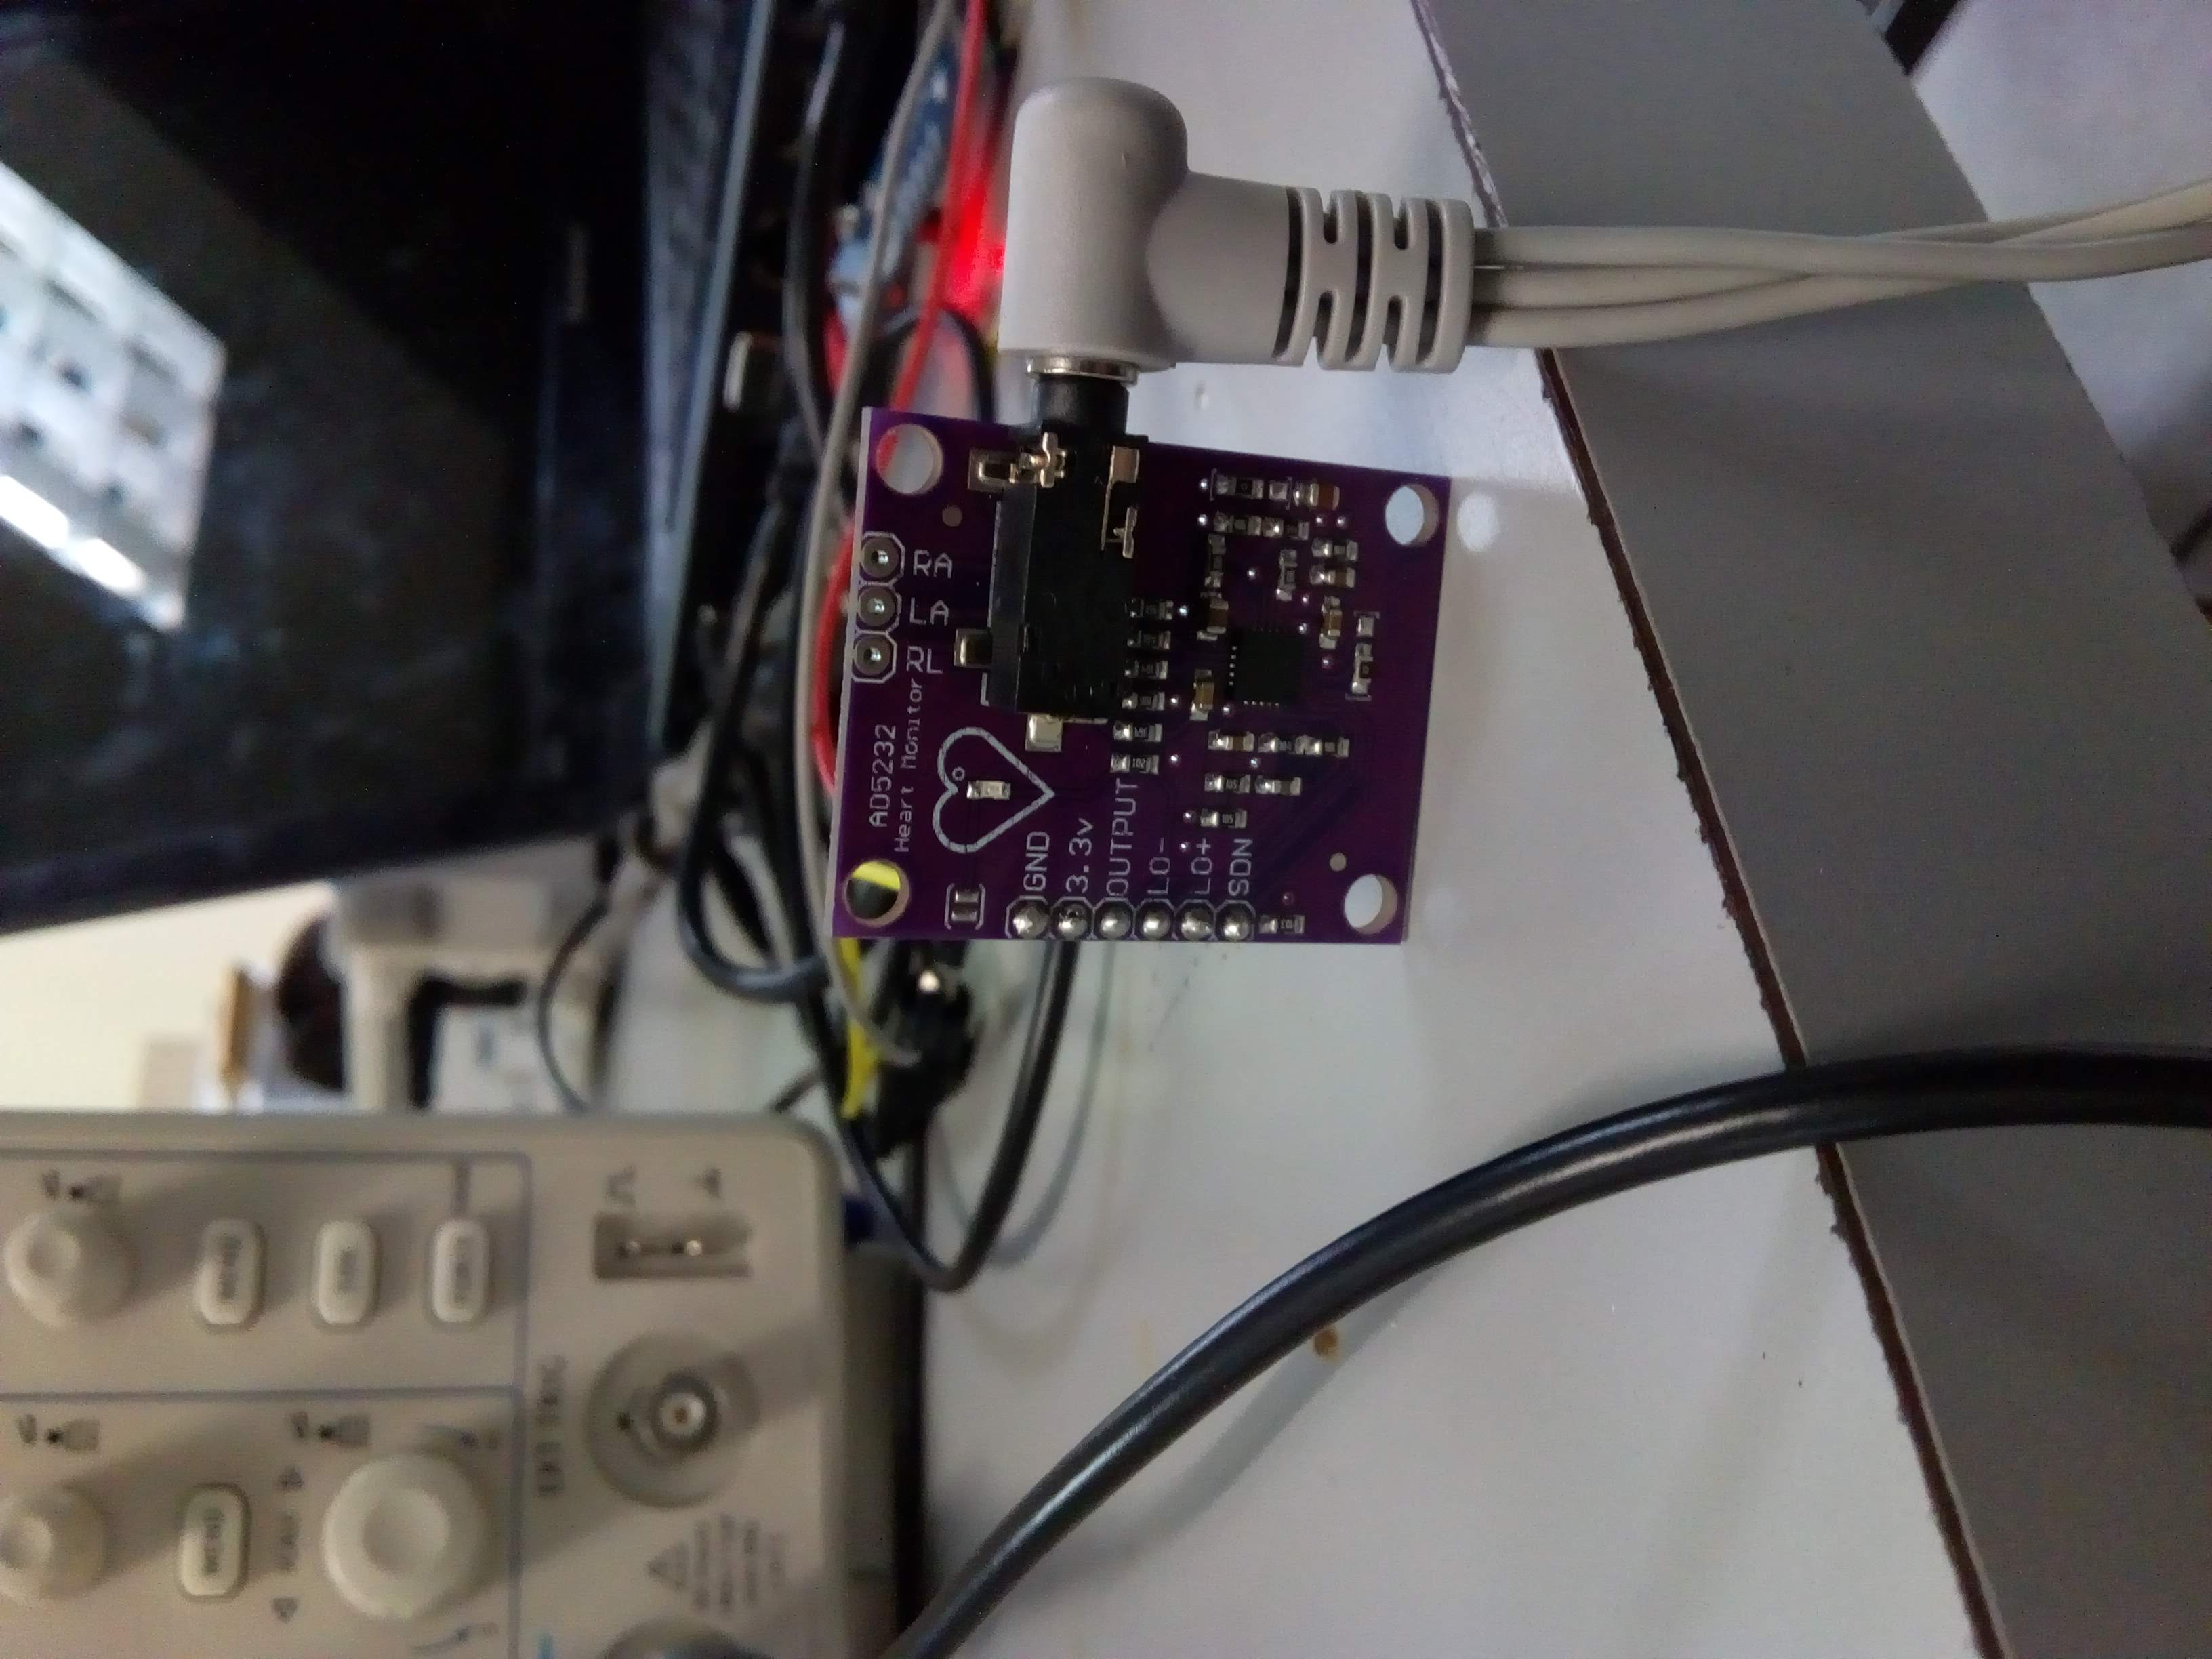
\includegraphics[width=0.6\textwidth]{AvancesPruebas/imagenes/AD8232-1.jpg}}
	\caption{Sensor de pulso AD8232.}
	\label{fig:AD8232Sensor}
\end{figure}


Una vez conectado correctamente, se colocaron los electrodos en el brazo derecho, brazo izquierdo y pierna derecha, respetando el color asignado a cada uno (verde, rojo y amarillo respectivamente) como se muestra en la figura \ref{fig:AD8232Electrodo}.\\
\begin{figure}[htbp!]
	\centering
	\fbox{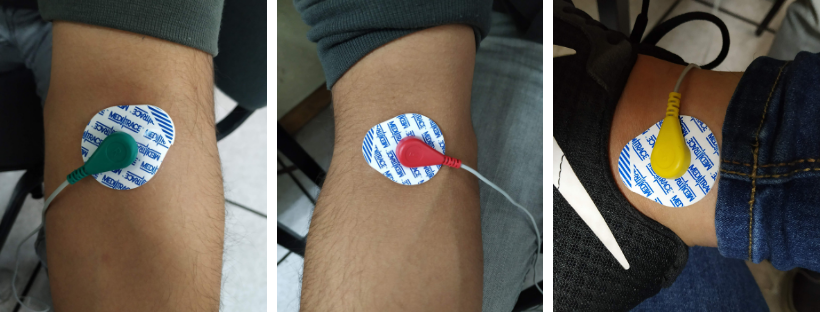
\includegraphics[width=0.7\textwidth]{AvancesPruebas/imagenes/AD8232-2.png}}
	\caption{Electrodos conectados el sensor de pulso AD8232.}
	\label{fig:AD8232Electrodo}
\end{figure}

La señal entregada por el sensor AD8232 se muestra en la figura \ref{fig:AD8232Osciloscopio}, a partir de esta señal podemos determinar que el sensor AD8232 proporciona una señal que puede ser útil para la detección de la frecuencia cardíaca, por lo que más adelante se realizarán pruebas con la señal digitalizada y procesada mediante un algoritmo.\\
\begin{figure}[htbp!]
	\centering
	\fbox{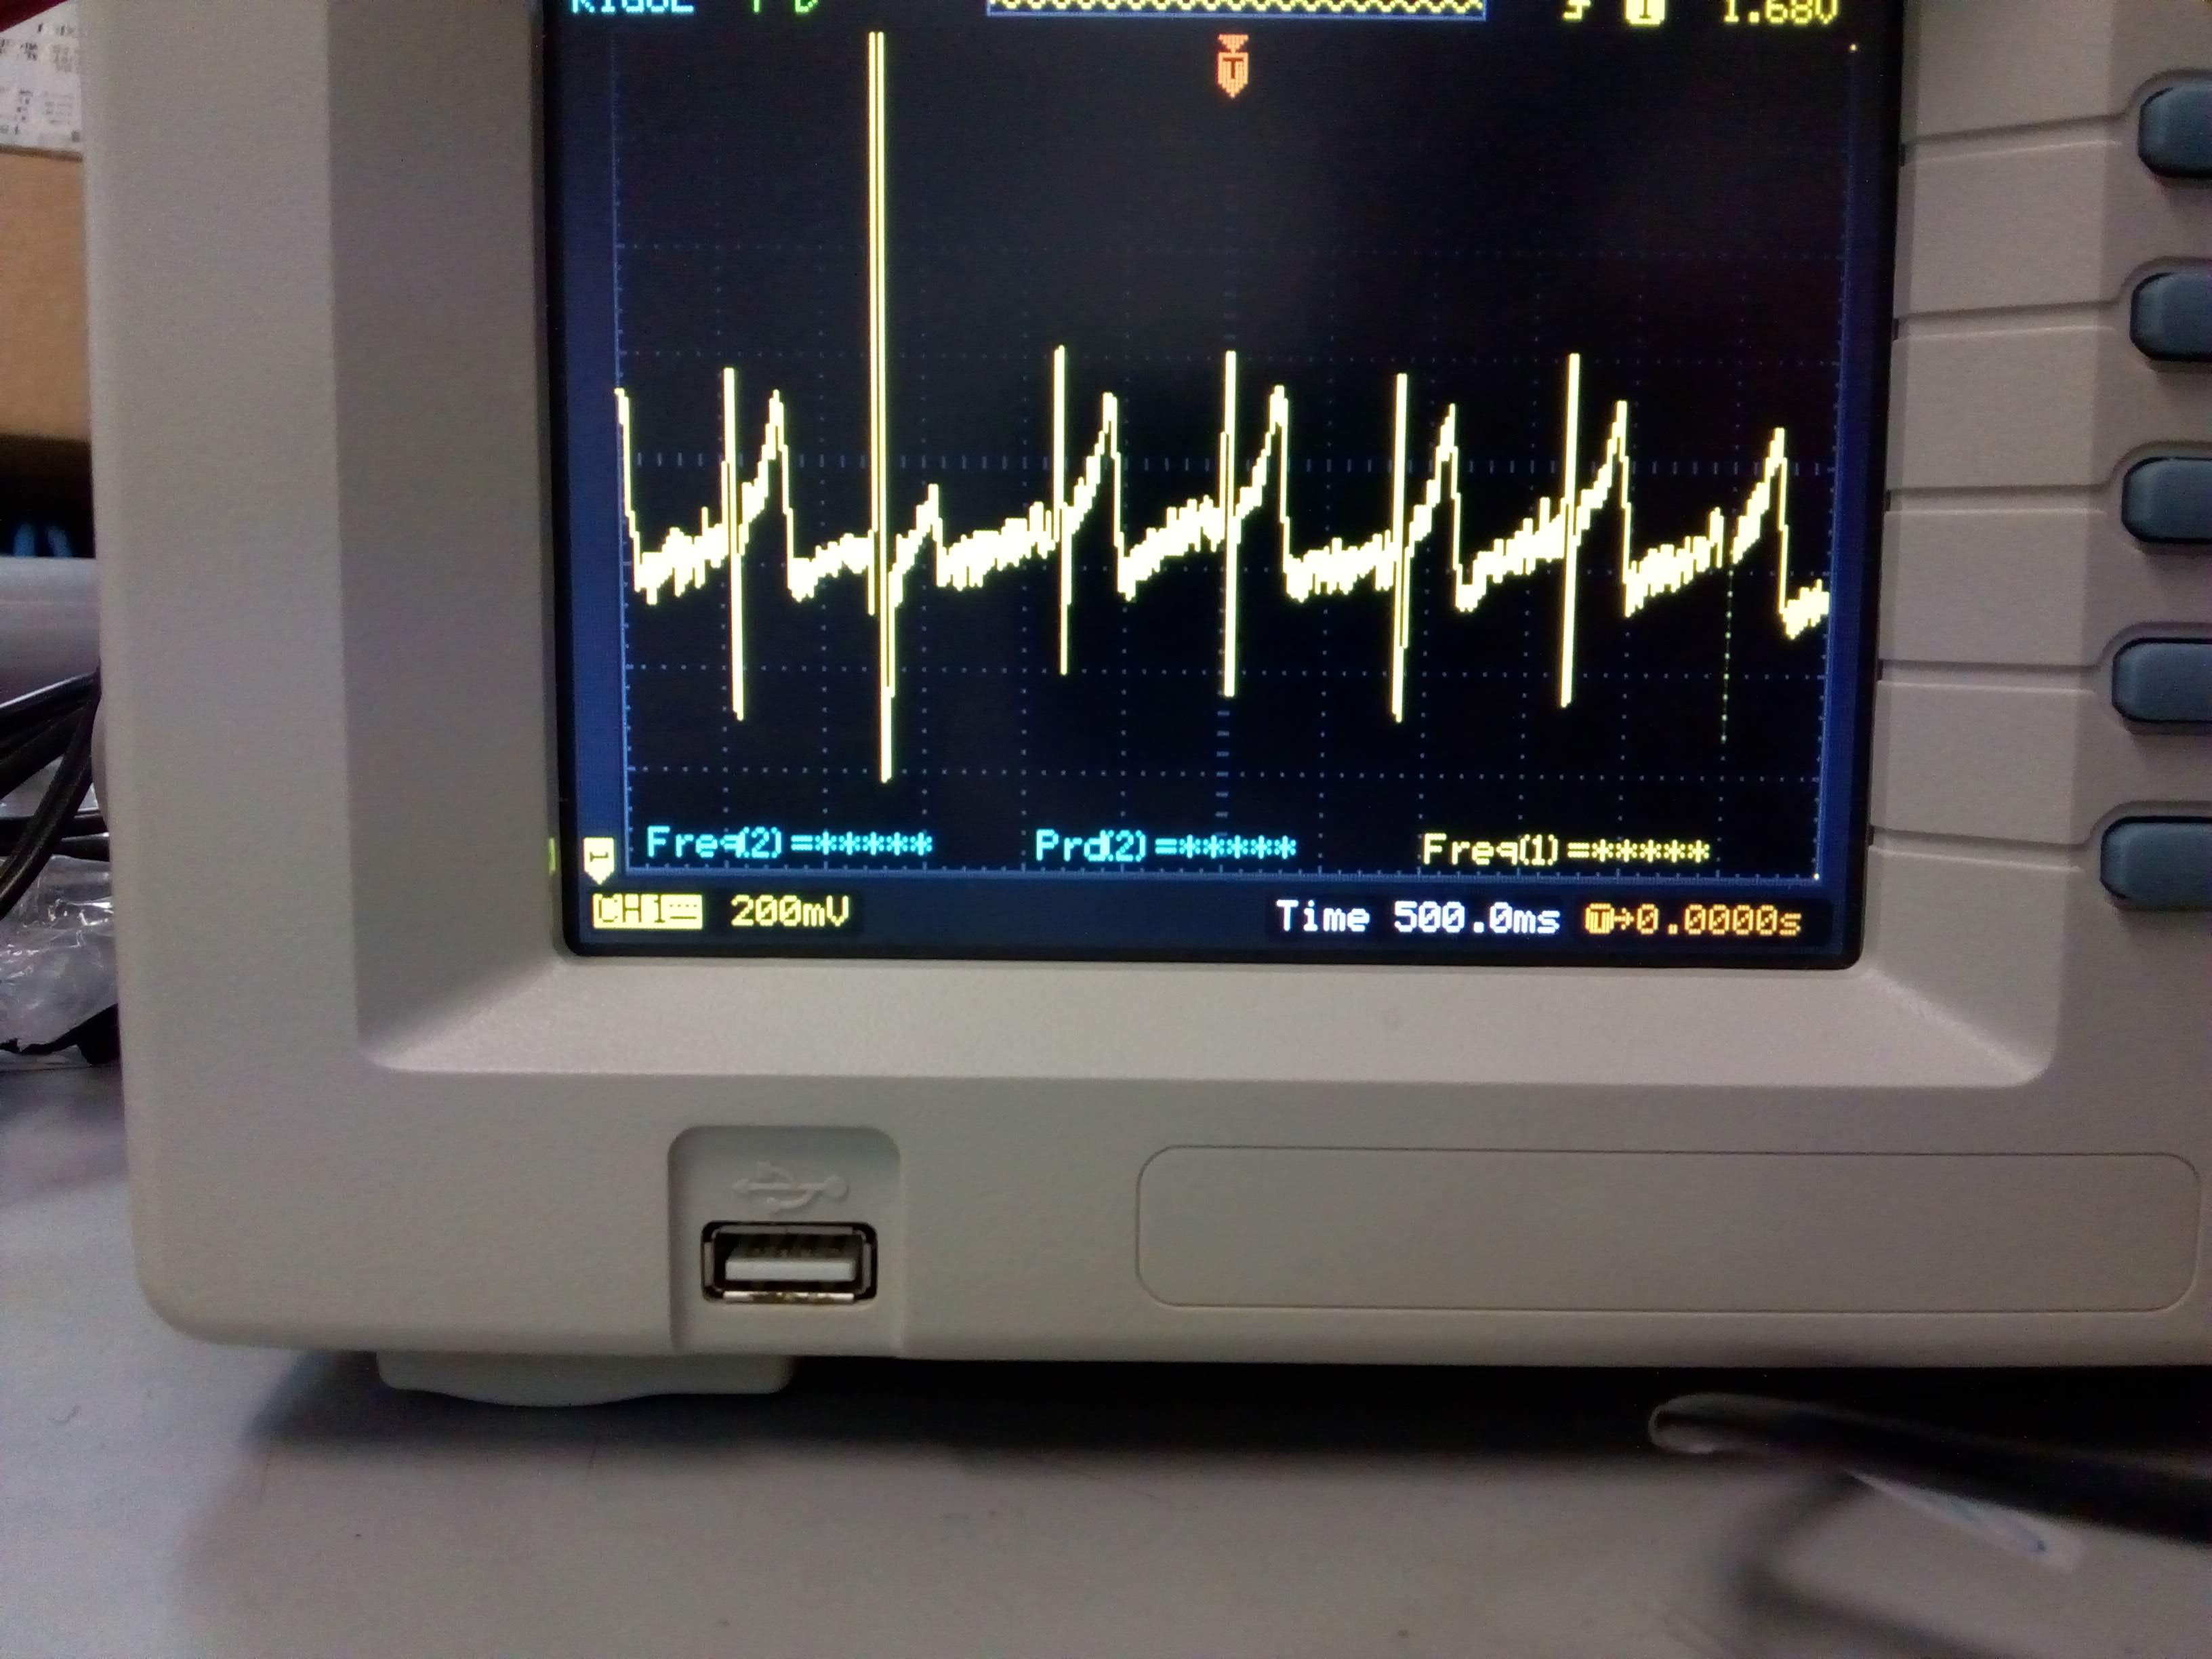
\includegraphics[width=0.6\textwidth]{AvancesPruebas/imagenes/AD8232-3.jpg}}
	\caption{Señal analógica del sensor de pulso AD8232.}
	\label{fig:AD8232Osciloscopio}
\end{figure}

\pagebreak

\subsection{Pulse sensor}
La prueba del sensor Pulse Sensor, fue realizado de manera similar al sensor anterior, sin embargo al ser un sensor fotopletismógrafo, se realizaron modificaciones al ambiente de pruebas utilizado.\\

Para esta prueba el sensor fue alimentado con 5V mediante las terminales indicadas en el sensor, al igual que en el sensor anterior, este fue alimentado haciendo uso de un módulo FT232 pero con un voltaje mayor. El sensor encendido se muestra en la figura \ref{fig:PulseSensor2}.

	\begin{figure}[htbp!]
		\centering
		\fbox{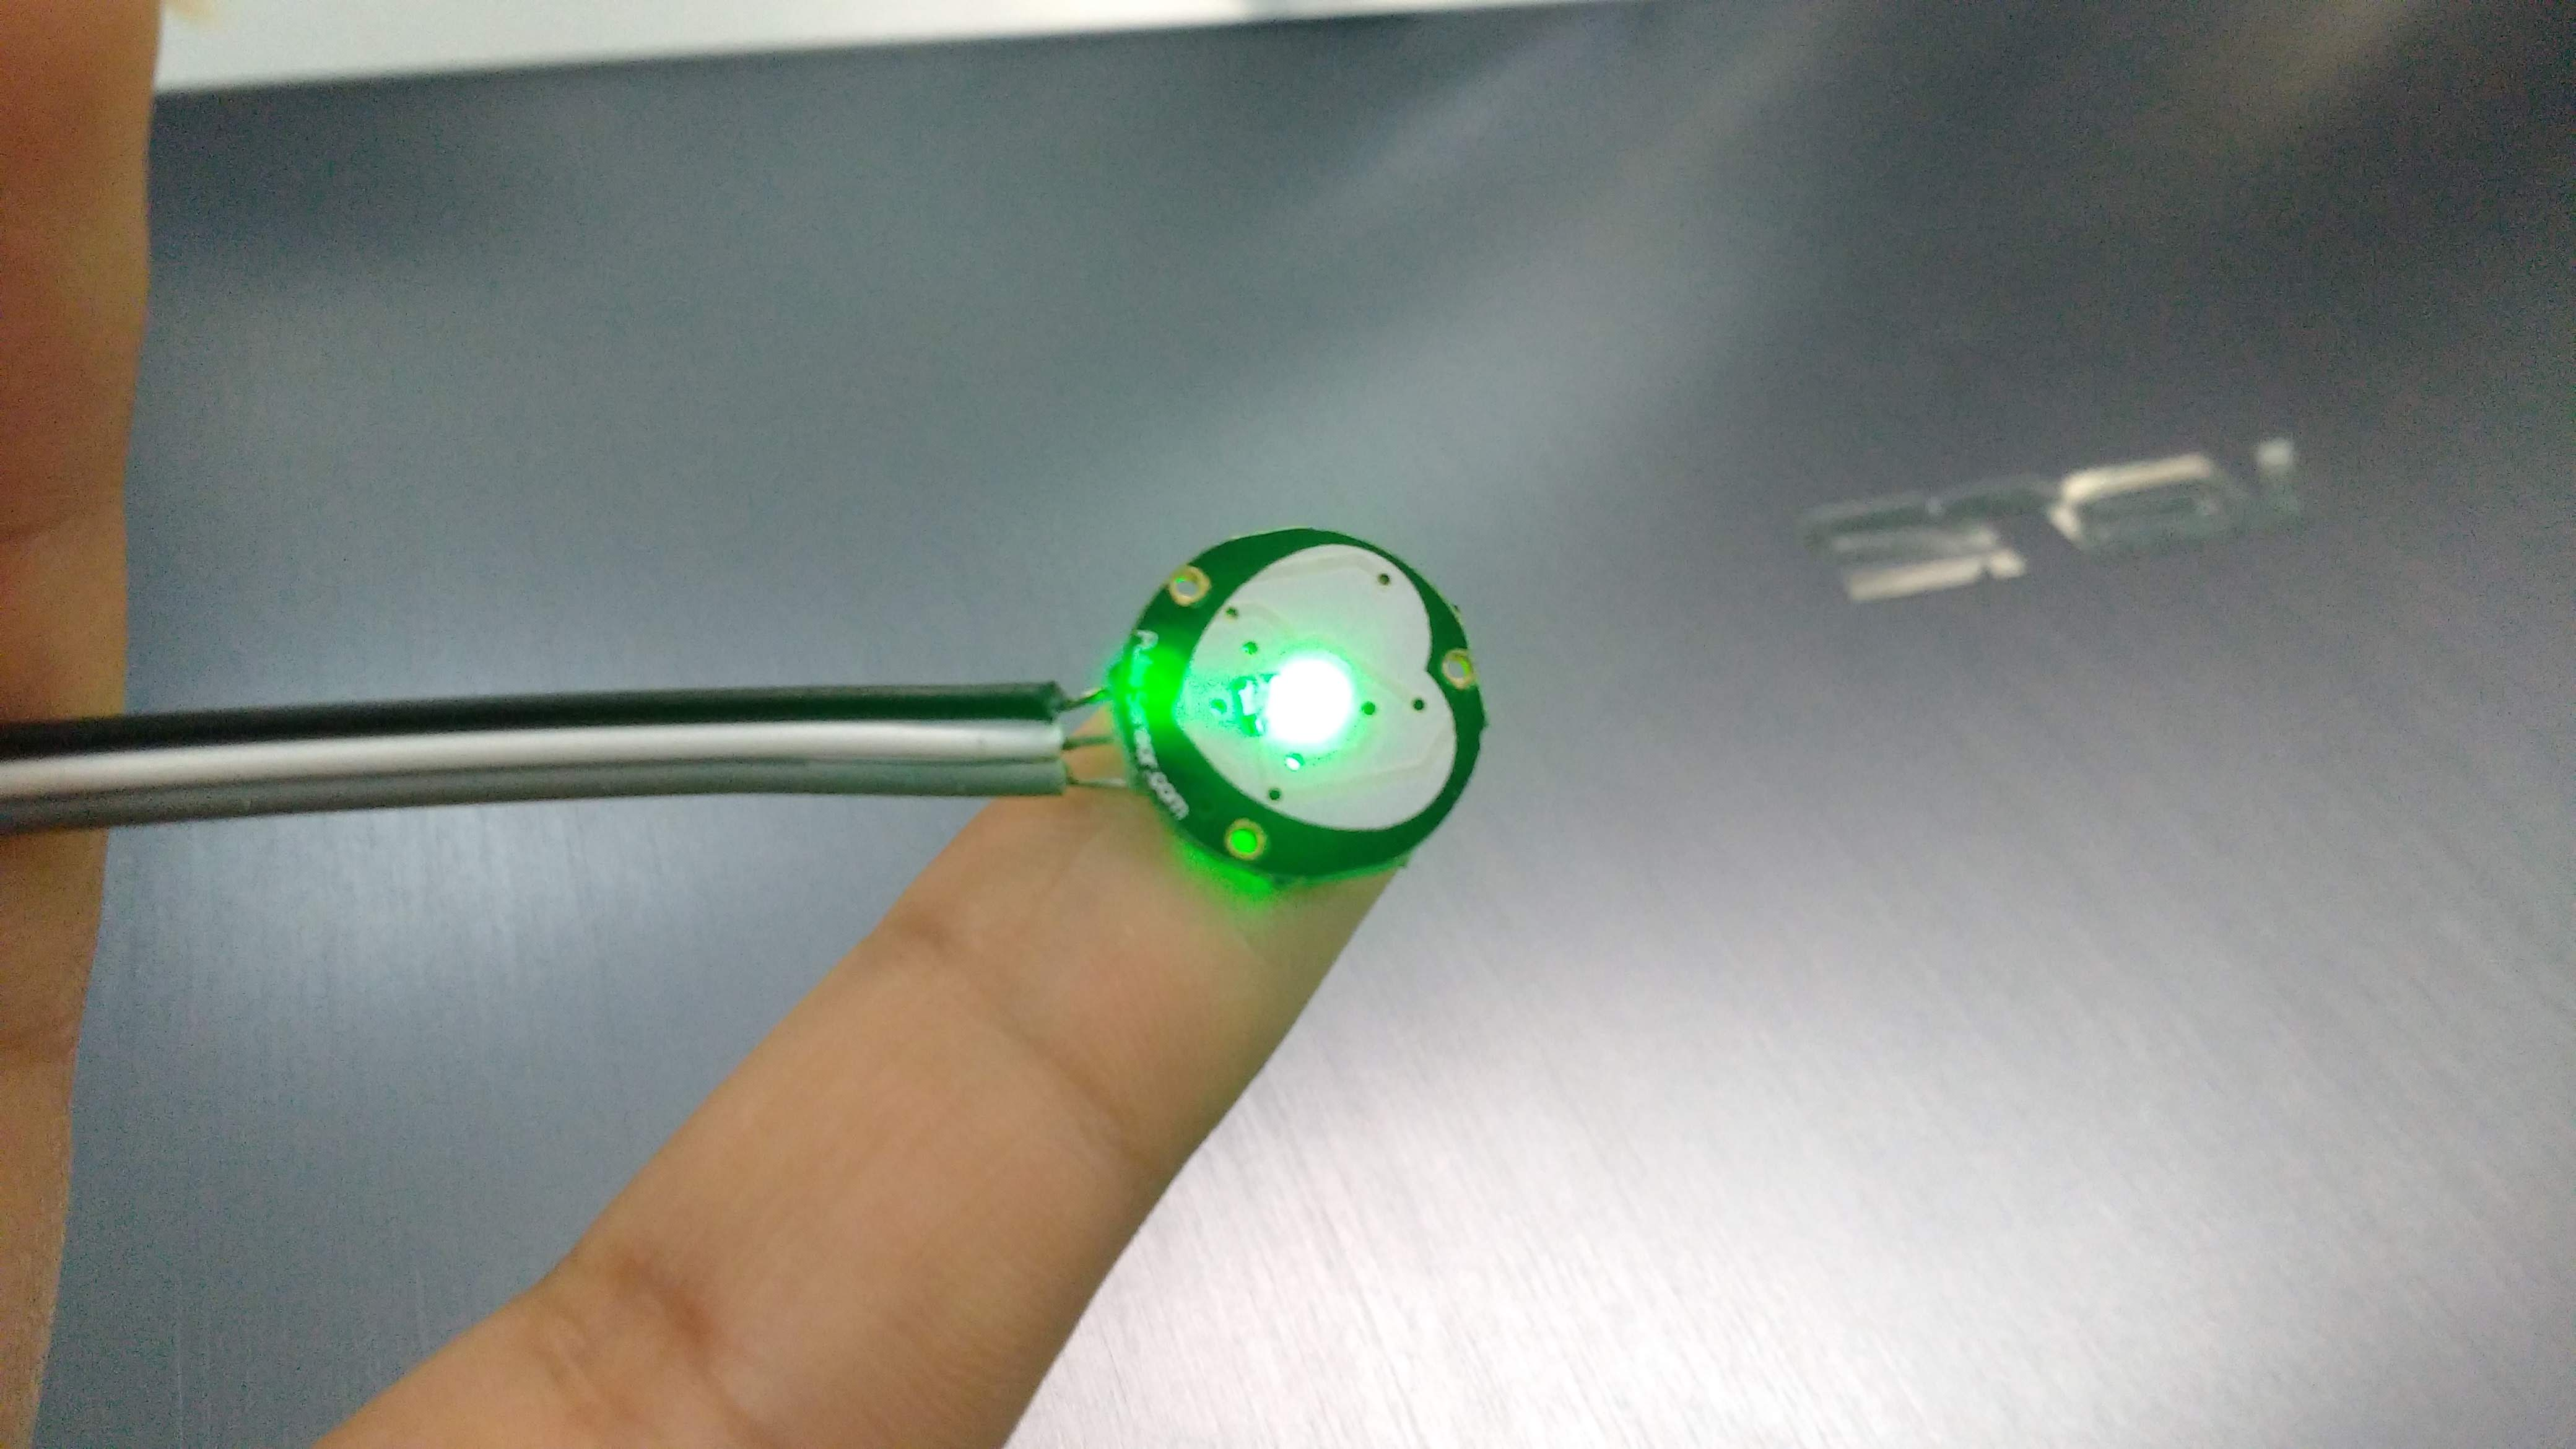
\includegraphics[width=0.65\textwidth]{AvancesPruebas/imagenes/PulseSensor2.jpg}}
		\caption{Sensor de pulso Pulse Sensor.}
		\label{fig:PulseSensor2}
	\end{figure}
	
Como el sensor es de tipo fotopletismógrafo, fue necesario aislar la luz emitida con el fin de evitar interferencias y que la señal pudiera ser medida correctamente. Para lograr esto, se colocó el sensor de pulso en el dedo índice de la mano y fue cubierto con un velcro negro, como se muestra en la figura \ref{fig:PulseSensor1}.\\
	
	\begin{figure}[htbp!]
		\centering
		\fbox{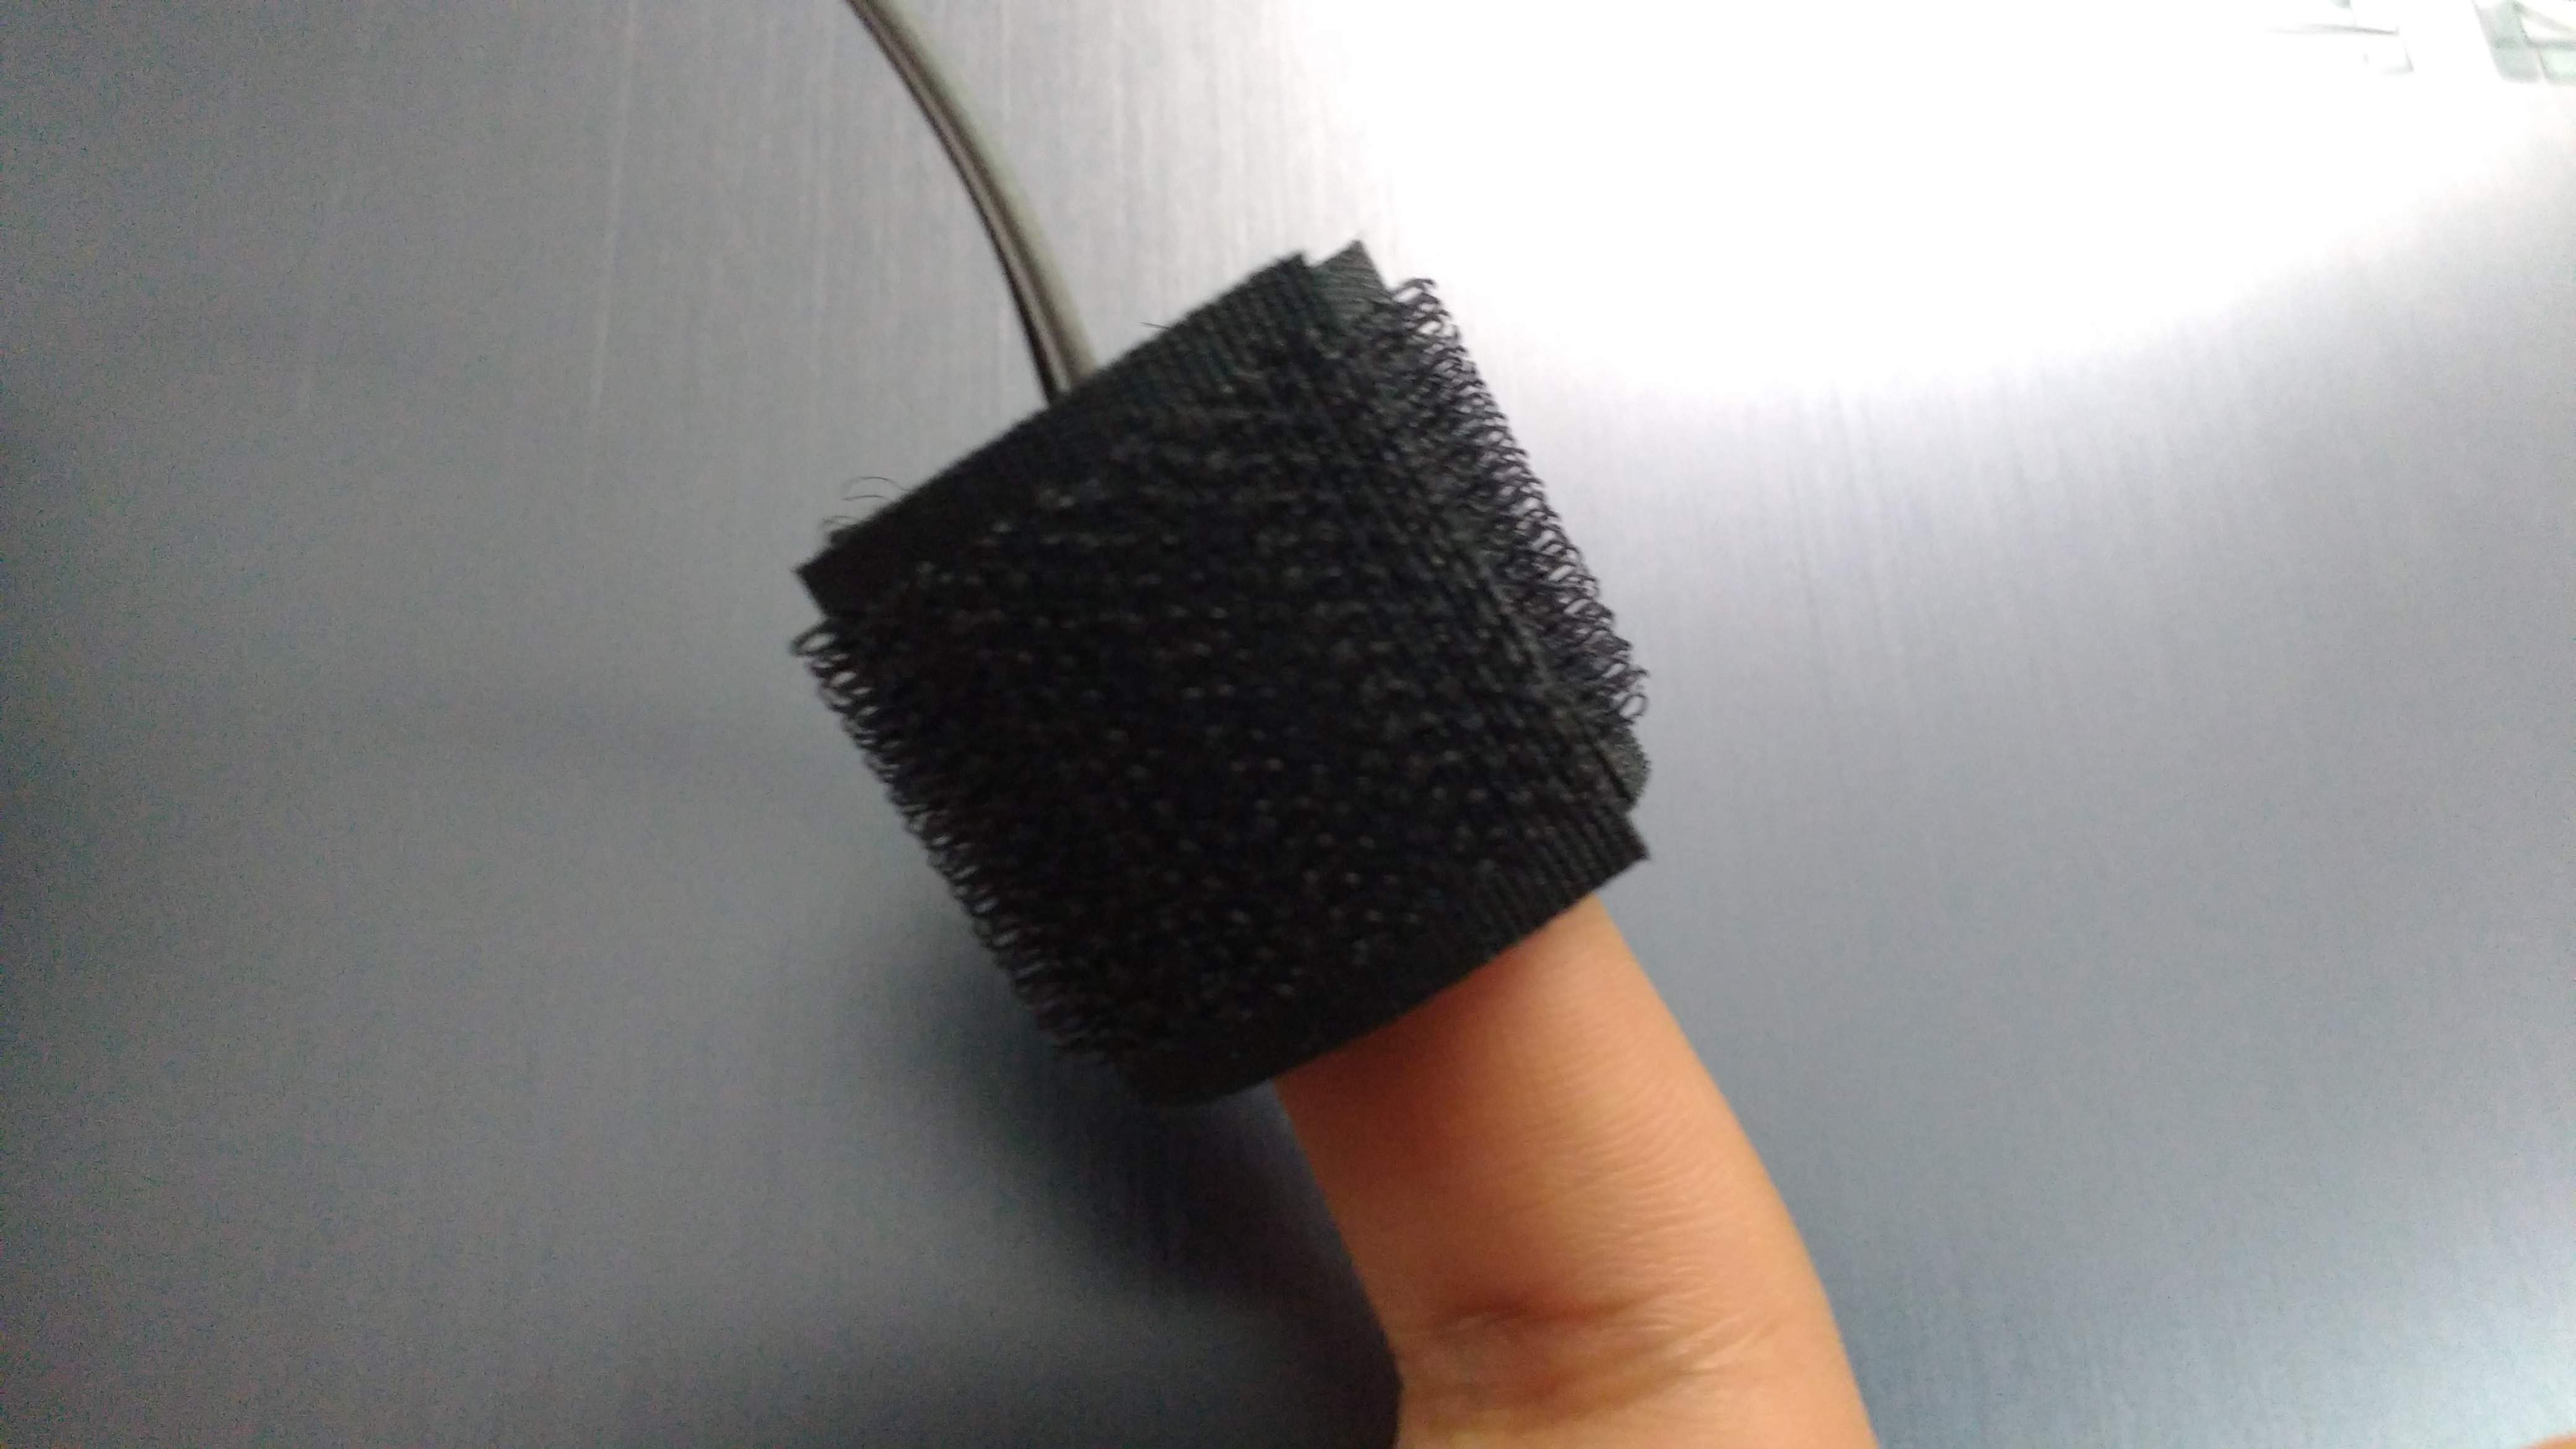
\includegraphics[width=0.6\textwidth]{AvancesPruebas/imagenes/PulseSensor1.jpg}}
		\caption{Prueba del sensor Pulse Sensor.}
		\label{fig:PulseSensor1}
	\end{figure}

La señal obtenida de este sensor se muestra en la figura \ref{fig:PulseSensor3}.	
	\begin{figure}[htbp!]
		\centering
		\fbox{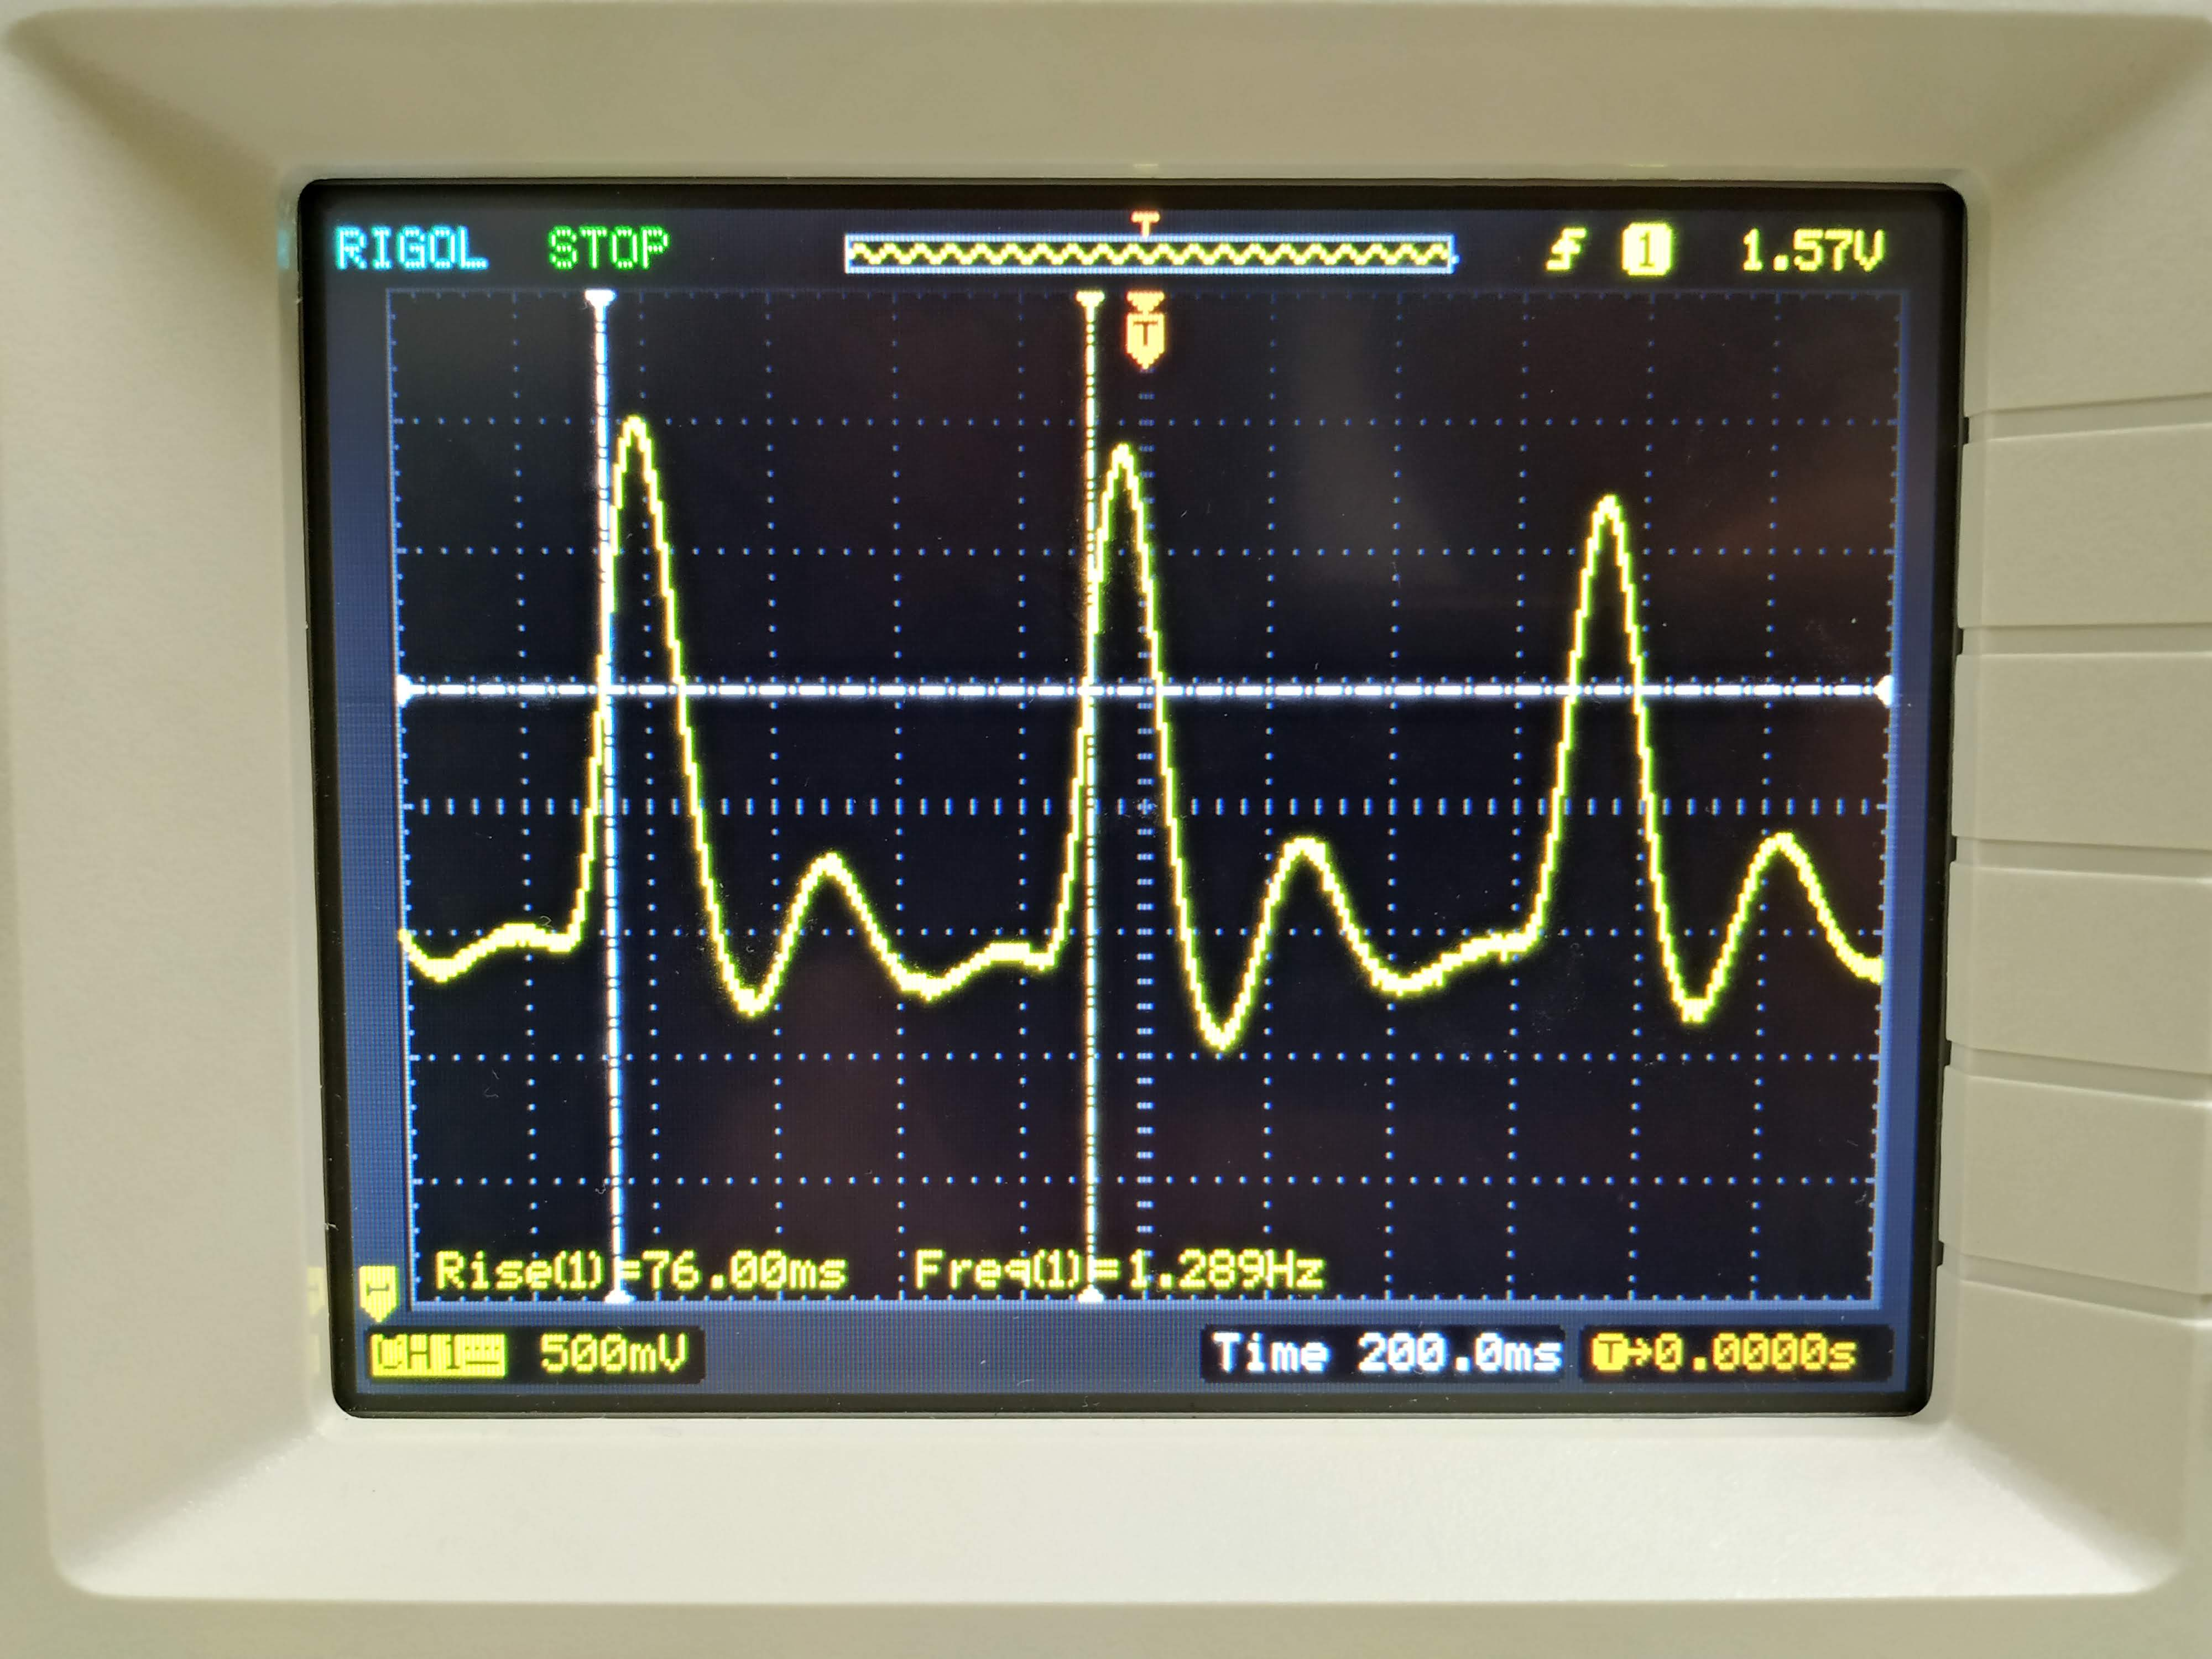
\includegraphics[width=0.6\textwidth]{AvancesPruebas/imagenes/PulseSensor3.jpg}}
		\caption{Señal analógica del sensor Pulse Sensor.}
		\label{fig:PulseSensor3}
	\end{figure}

\pagebreak \newpage	
\section{Digitalización de señal analógica}
Una vez obtenidas las señales analógicas de cada sensor, se realizaron los programas en lenguaje c y ensamblador necesarios para digitalizar ambas señales haciendo uso del convertidor analógico digital del dsPIC.\\

En la figura se muestra el diagrama de flujo para la configuración de los puertos, ADC y UART del microcontrolador. En el diagrama se pueden observar los diferentes paso realizados para configurar el microcontrolador y así poder obtener y procesar la señal medida de los sensores de pulso.

A continuación se describen las etapas del diagrama de flujo junto con el código correspondiente para su realización.

\begin{enumerate}
	\item \textbf{Configuración de puertos:} Esta rutina inicializa los periféricos del microcontrolador,indicando qué puertos serán considerados como entradas o salidas. En este caso, las entradas que tendrá el microcontrolador son el pin B2,que funcionará como entrada analógica para la salida del sensor de pulso y el pin C14 el cuál es el transmisor TX del UART. Para el caso de las salidas, se configuró el pin C13 el cual es el receptor del UART. 
	
	\lstset{language=c}
	El código de la configuración de puertos se describe a continuación:
	\begin{lstlisting}[frame=single]
	void iniPerifericos( void )
	{
        PORTA=0;
		Nop();
		TRISA=0;
		Nop();
		LATA=0;
		PORTB = 0;
		Nop();
		LATB = 0;
		Nop();
		TRISBbits.TRISB0=1;
		Nop();
		TRISBbits.TRISB1=1;
		Nop();
		TRISBbits.TRISB2=1;
		Nop();
		PORTC=0;
		Nop();
		TRISCbits.TRISC13=0;
		Nop();
		TRISCbits.TRISC14=1;
		Nop();
	}
	\end{lstlisting}
	
%	\item \textbf{Configuración de reloj para ADC:} Se configura el
	
	\item \textbf{Configuración UART:} Esta rutina configura el UART indicando que obtendrá los datos de los sensores de pulso a través de los pines configurados para eso. En esta sección se incluyen también las interrupciones correspondientes al UART.
	\begin{lstlisting}[frame=single]
	void configurarUART1()
	{
		/*Inicializar el uart1*/
		U1MODE=0X0420;
		U1STA=0X8000;
		U1BRG=5;
	}
	\end{lstlisting}
	
	\item \textbf{Configuración de ADC:} Incluye la rutina donde se configura el ADC para su uso. En esta sección se especifica que el pin de entrada B2 será el canal de entrada para la conversión analógico digital. Así mismo se realiza la especificación de las interrupciones correspondientes al ADC.
	
	\lstset{language=c}
	El código de la configuración del ADC se describe a continuación:
	\begin{lstlisting}[frame=single]
	void configurarADC()
	{
		ADCON1=0x0044;
		ADCON2=0x0000;
		ADCON3=0x0F02;
		ADCHS=0x0002;
		ADPCFG=0xFFF8;
		ADCSSL=0x0000;
	}
	\end{lstlisting}

\end{enumerate}

	\begin{figure}[htbp!]
		\centering
		\fbox{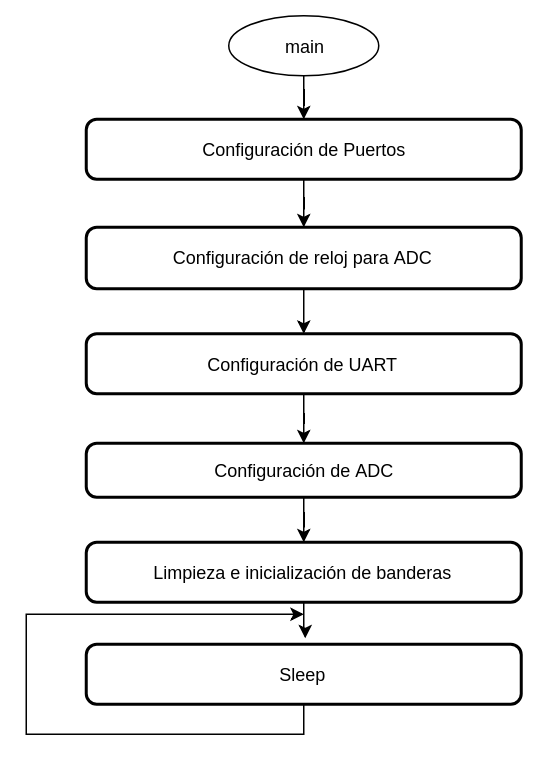
\includegraphics[width=0.4\textwidth]{AvancesPruebas/imagenes/ConfiguracionMicro.png}}
		\caption{Diagrama de flujo del programa de configuración del dsPIC40F4013.}
		\label{fig:ConfiguracionMicro}
	\end{figure}
\pagebreak
En la figura \ref{fig:FlujoSerial} se muestra el diagrama de flujo para la obtención de los datos digitalizados por el convertidor analógico digital y así como el proceso llevado a cabo para graficar los datos obtenidos.\\

A continuación se describen las etapas del diagrama de flujo junto con el código correspondiente para su realización.

\begin{enumerate}
	\item \textbf{Configuración de interfaz serie:} Esta función configura los elementos de la interfaz serie como el nombre del dispositivo serial a usar y la velocidad de comunicación en baudios.
	\item \textbf{Creación/apertura de archivo:} En este paso se crea o abre un archivo en el cuál se escribirán los datos leídos a través de la interfaz serie.
	\item \textbf{Obtención de datos de la interfaz serie:} Lee los datos que están siendo enviados por UART a través de la interfaz serie configurada anteriormente.
	\item \textbf{Cierre de archivo:} Una vez leídos todos los datos por UART, se cierra el archivo en donde se realizó la escritura de los mismos.
	\item \textbf{Gráfica de señal digitalizada:} Se muestra una gráfica a partir del archivo creado usando el programa gnuplot, en donde puede verse la señal convertida.
\end{enumerate}
\pagebreak
\lstset{language=c}
Código para obtención y graficación de datos obtenidos a través de la interfaz serial.

{\small 
\begin{lstlisting}[frame=single]
#include <stdio.h>
#include <stdlib.h>
#include <termios.h>
#include <unistd.h>
#include <fcntl.h>

#define N  1024
#define EVER 1
char cad[20];
int fd_serie=0;
int config_serial ( char *, speed_t );
int config_serial( char *dispositivo_serial, speed_t baudios );

int main()
{
	FILE *archivo;
	archivo=fopen("prueba.txt","w+");
	fd_serie = config_serial( "/dev/ttyUSB0", B19200 );
	printf("Procesando datos de el ADC\n");
	unsigned char cad=' ';
	int entrada=0;
	unsigned int prueba=0;
	//int muestras[4096];
	int i;
	for(i = 0; i<1500; i++)	//DATOS A LEER
	{
		printf("FOR\n");
		if(read(fd_serie,&cad,1) == 0)
		printf(" --> \n");
		
		printf("% x\n", cad);
		
		printf("Valor total=% d\n",prueba);
		fprintf(archivo,"% d % d\n",i,cad );
	}
	close( fd_serie );
	fclose(archivo);
	system("./gnuplot");
	return 0;
}

int config_serial( char *dispositivo_serial, speed_t baudios )
{
	struct termios newtermios;
	int fd;
	
	newtermios.c_cflag 	= CBAUD | CS8 | CLOCAL | CREAD;
	newtermios.c_iflag 	= IGNPAR;
	newtermios.c_oflag	= 0;
	newtermios.c_lflag 	= TCIOFLUSH | ~ICANON;
	newtermios.c_cc[VMIN]	= 1;
	newtermios.c_cc[VTIME]	= 0;
	
	// Configura la velocidad de salida del UART
	if( cfsetospeed( &newtermios, baudios ) == -1 )
	{
	  printf("Error al establecer velocidad de salida \n");
      exit( EXIT_FAILURE );
	}
	// Configura la velocidad de entrada del UART
	if( cfsetispeed( &newtermios, baudios ) == -1 )
	{
	  printf("Error al establecer velocidad de entrada \n" );
	  exit( EXIT_FAILURE );
	}
	// Limpia el buffer de entrada
	if( tcflush( fd, TCIFLUSH ) == -1 )
	{
	  printf("Error al limpiar el buffer de entrada \n" );
	  exit( EXIT_FAILURE );
	}
	// Limpia el buffer de salida
	if( tcflush( fd, TCOFLUSH ) == -1 )
	{
	  printf("Error al limpiar el buffer de salida \n" );
	  exit( EXIT_FAILURE );
	}

	if( tcsetattr( fd, TCSANOW, &newtermios ) == -1 )
	{
      printf("Error al establecer los parametros\n" );
	  exit( EXIT_FAILURE );
	}
	//Retorna el descriptor de archivo
	return fd;
}
\end{lstlisting}
}
Diagrama de flujo para la obtención de datos de la interfaz serial.
	\begin{figure}[htbp!]
		\centering
		\fbox{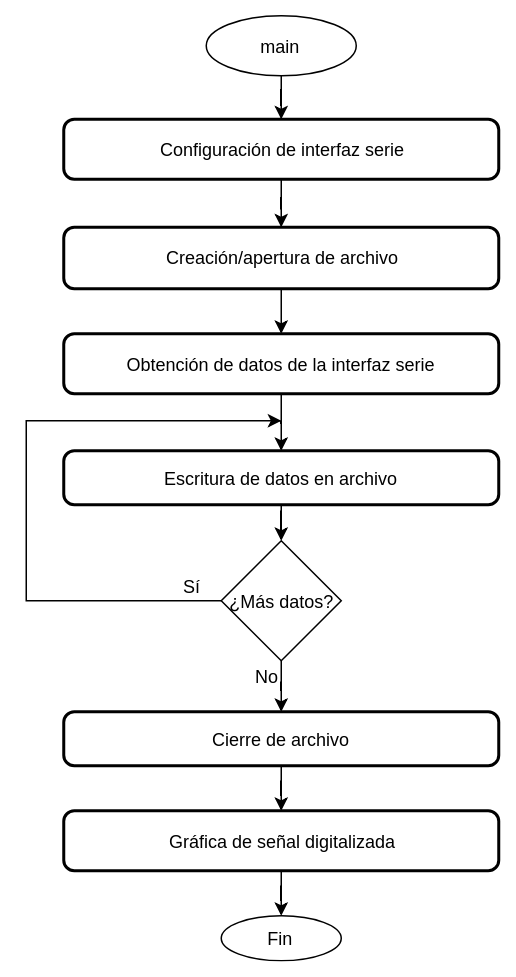
\includegraphics[width=0.4\textwidth]{AvancesPruebas/imagenes/Serial.png}}
		\caption{Diagrama de flujo de la obtención de señal digitalizada.}
		\label{fig:FlujoSerial}
	\end{figure}
\pagebreak
		
Con los programas listos, se realizó la conexión de cada uno de los sensores para verificar el  correcto funcionamiento del convertidor analógico digital y obtener el archivo y gráfica de la señal de cada sensor.\\

El primer sensor que fue conectado fue el AD8232, el diagrama de conexión se muestra en la figura \ref{fig:ConexionAD8232}. En ella se puede observar que la única entrada que tiene el microcontrolador para esta prueba es en el pin B2, el cual es tomado como entrada analógica y es de donde el ADC tomará los datos para convertirlos.\\

Es importante aclarar que este sensor fue alimentado con 3.3 V.\\

	\begin{figure}[htbp!]
		\centering
		\fbox{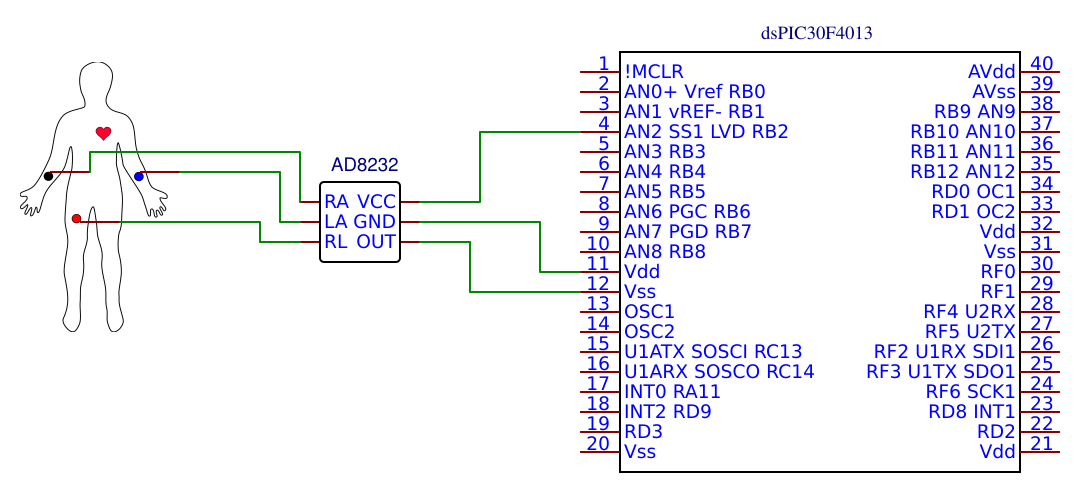
\includegraphics[width=0.95\textwidth]{AvancesPruebas/imagenes/AD8232Conexion.png}}
		\caption{Conexión de AD8232 con dsPIC30F4013.}
		\label{fig:ConexionAD8232}
	\end{figure}
	
El resultado de la ejecución, así como la gráfica obtenida de la señal digital se muestran en las figuras \ref{fig:TerminalAD8232} y \ref{fig:GraficaAD8232} respectivamente.\\

	\begin{figure}[htbp!]
		\centering
		\fbox{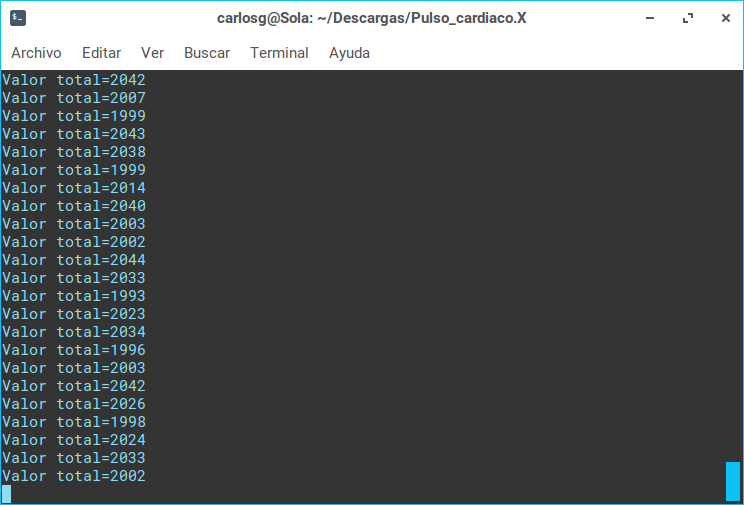
\includegraphics[width=0.6\textwidth]{AvancesPruebas/imagenes/terminalAD8232.png}}
		\caption{Resultado de ejecución para sensor AD8232.}
		\label{fig:TerminalAD8232}
	\end{figure}
	
	\begin{figure}[htbp!]
		\centering
		\fbox{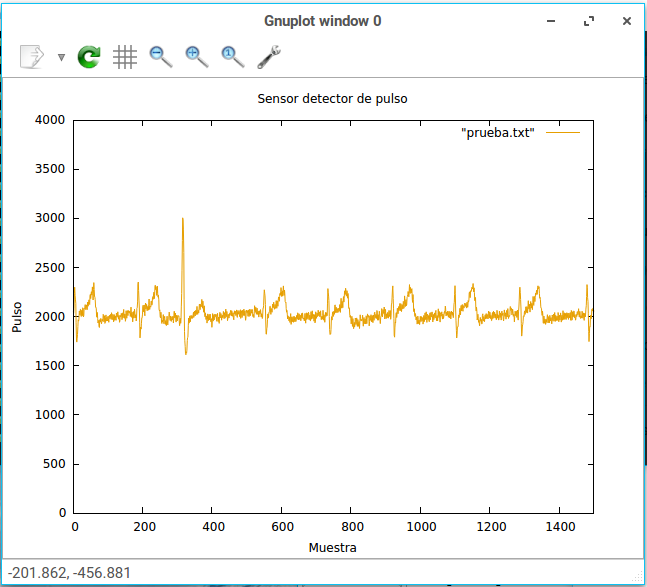
\includegraphics[width=0.6\textwidth]{AvancesPruebas/imagenes/graficaAD8232.png}}
		\caption{Gráfica de señal del sensor AD8232.}
		\label{fig:GraficaAD8232}
	\end{figure}
	
Al igual que el sensor AD8232, el sensor Pulse Sensor fue conectado directamente a la entrada AN2 del microcontrolador para que fuera procesada y transformada por el ADC, sin embargo, este sensor sí necesita ser alimentado con 5V.\\

En la figura \ref{fig:ConexionPulseSensor} se muestra el diagrama de conexión del microcontrolador con el sensor.\\
	
	\begin{figure}[htbp!]
		\centering
		\fbox{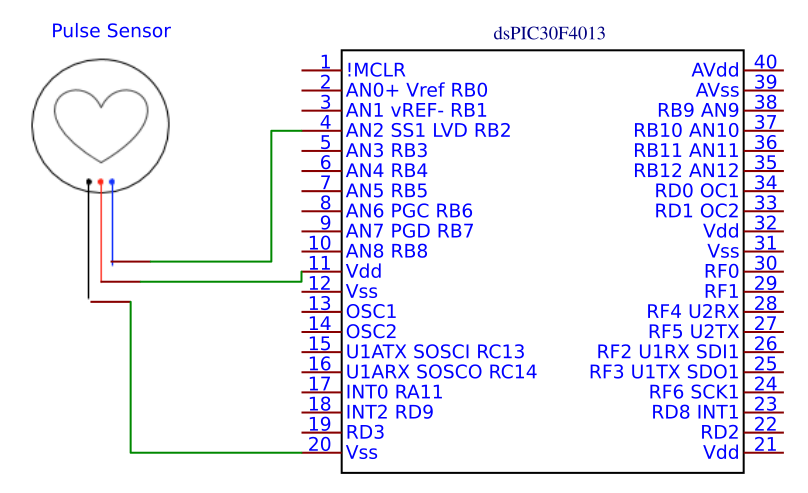
\includegraphics[width=0.7\textwidth]{AvancesPruebas/imagenes/PulseSensorConexion.png}}
		\caption{Conexión de PulseSensor con dsPIC30F4013.}
		\label{fig:ConexionPulseSensor}
	\end{figure}

Para la transmisión de los datos convertidos hacia la computadora, se implementó el mismo código que para el sensor anterior. El resultado de la ejecución para este sensor se muestra en las figuras \ref{fig:TerminalAD8232} y \ref{fig:GraficaPulseSensor}.
	
	\begin{figure}[htbp!]
		\centering
		\fbox{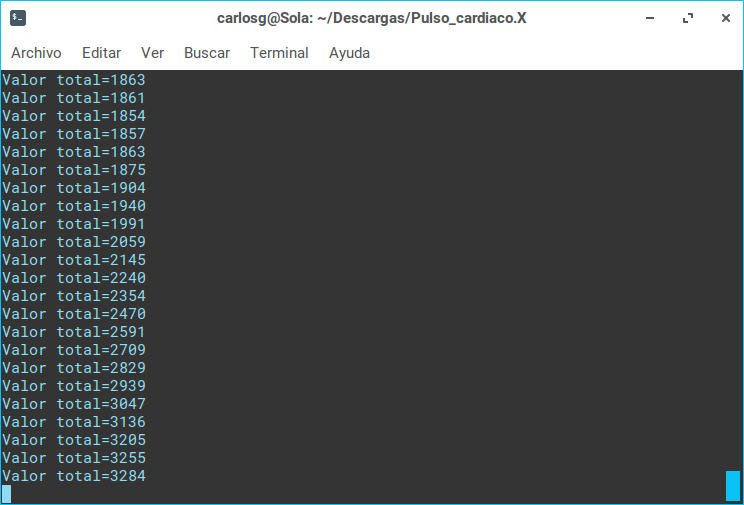
\includegraphics[width=0.6\textwidth]{AvancesPruebas/imagenes/terminalPulseSensor.png}}
		\caption{Resultado de ejecución para sensor Pulse Sensor.}
		\label{fig:TerminalPulseSensor}
	\end{figure}
	
	\begin{figure}[htbp!]
		\centering
		\fbox{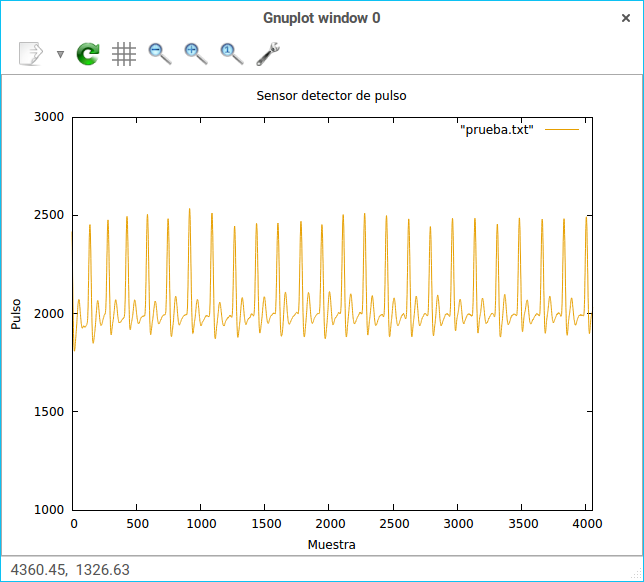
\includegraphics[width=0.6\textwidth]{AvancesPruebas/imagenes/graficaPulseSensor.png}}
		\caption{Gráfica de señal del sensor Pulse Sensor.}
		\label{fig:GraficaPulseSensor}
	\end{figure}
	
	\clearpage